\chapter{A LUZ COMO MATERIAL E O CUBO PRETO}

Segundo \citeonline[p. 1]{azevedo} a problemática da luz atravessa a história da arte, de finais do século XIX e durante o século XX. A função da luz não é mais somente de iluminar, de tornar visível uma obra ou um objeto, ou o mero reflexo dos seus efeitos suspensos no espaço. A luz passa a ser tratada como objeto ou material. Na perspectiva da arte contemporânea, se vê que, em muitas obras, a luz passa à matéria. \citeonline[p. 50]{brandi} destaca que "alguns artistas e movimentos estéticos estão fortemente relacionados com a linguagem da luz, mesmo quando não a utilizam como objeto central da obra". 

De acordo com \citeonline[p. 18]{vega} os artistas, em diferentes épocas, se viram inspirados e cativados pela luz, tanto a natural quanto a artificial, e tentaram capturar seu mistério e sua natureza mágica em suas criações. Alguns em particular, como Caravaggio, Vermeer e Monet, buscaram retratar, quase como uma obsessão, a luz e seus efeitos no mundo ao seu redor e, mais recentemente, os artistas contemporâneos vem se utilizando da luz como matéria-prima, realizando manipulações em três dimensões para projetar suas dimensões infinitas. \citeonline[p. 23]{vega} afirma também que, atualmente, muitos artistas exploram as possibilidades da luz artificial, trabalhando com mescla de materiais e diversos tipos de fontes de luz. 

James Turrell, por exemplo, foi pioneiro de uma nova preocupação com os fenômenos do espaço e da luz. Em seus primeiros trabalhos investigou os efeitos da luz artificial. Ele também desenvolveu várias instalações que aumentaram a relação entre a luz e a estrutura arquitetônica. Em conversa com \citeonline[p. 114]{adcock}, ele relata que uma das dificuldades de usar a luz é que ainda não é tradição utilizá-la em nossa cultura. Por outro lado, não é mais incomum usá-la do que usar pedra, argila, aço ou tinta. O artista declara seu interesse em trabalhar a luz como material, mas não luz em vidro, fibra de vidro ou acrílico, e sim no próprio espaço e nas qualidades do espaço, fazendo luz sem a forma física tradicional. Ele nos traz também que há uma rica tradição na pintura do trabalho sobre a luz, mas que isso de fato não é luz - é o registro da visão. Na figura \ref{fig:james_turrell} podemos ver sua obra entitulada \textit{The light inside} que transforma as paredes de um túnel em vasos para a condução da luz e nos dá uma ideia da dimensão na qual o artista trabalha este material. 

\begin{figure}[H]
    \centering
    \caption{The light inside, James Turrell, 1999}
	\vspace*{0,2cm}
    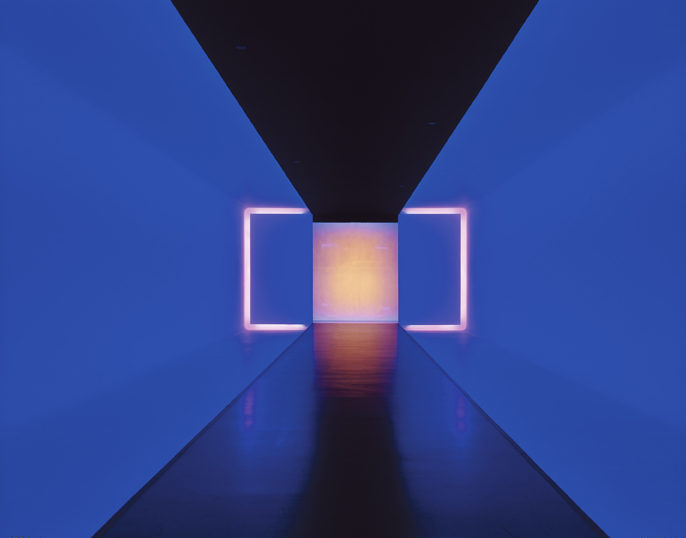
\includegraphics[width=0.8\textwidth]{./04-figuras/james_turrell}
    \label{fig:james_turrell}
\end{figure}
\vspace*{-0,9cm}
{\raggedright \fonte{Disponível em: <http://jamesturrell.com/work/thelightinside/>. Acesso em: 18 jun. 2018}}\\


Outro artista cuja obra é relevante no contexto deste trabalho e que, além da luz, explora a perspectiva da arte computacional, é o japonês Takahito Matsuo que, segundo \citeonline[p. 5]{soares}, cria mundos interativos de fantasia e de luz que fazem parte de uma estética enigmática, misturando som e luz perante os movimentos do observador. Seu trabalho destaca as diferentes gradações de luz e sombra que contrastando mostram um mundo de fantasia e imaginação. Em \textit{Fantasias Aquáticas Iluminadas} (figura \ref{fig:takahito_matsuo}), a exploração através de luz, projeções, arquitetura e interações humanas é fortemente encorajada. À medida que os visitantes se aproximam das paredes, se movimentam e se afastam, o número e a frequência das medusas aumentam e diminuem. As formas orgânicas e a brilhante paleta de azúis criam um mundo subaquático surreal, onde movimentos lúdicos e interações com o espaço arquitetônico resultam em uma comunicação não dita entre artista e participante. 

\begin{figure}[H]
    \centering
    \caption{Fantasias Aquáticas Iluminadas, Takahito Matsuo, 2009}
	\vspace*{0,2cm}
    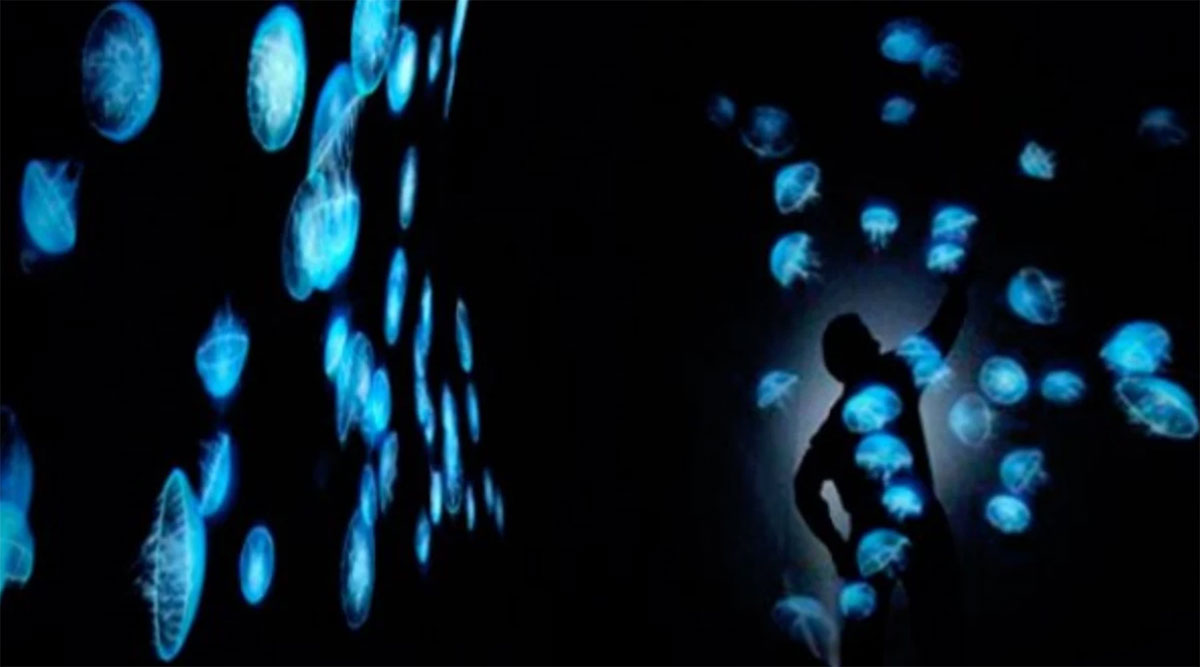
\includegraphics[width=0.8\textwidth]{./04-figuras/takahito_matsuo}
    \label{fig:takahito_matsuo}
\end{figure}
\vspace*{-0,9cm}
{\raggedright \fonte{\citeonline{soares}}}\\

Já o trabalho de Jim Campbell chama à atenção pela antítese presente em suas obras. Em um vídeo produzido pela \citeonline{kqed}, o artista constata que em um mundo de alta definição e telas cada vez mais finas usa tecnologia para produzir o contrário: imagens borradas e em baixa resolução em painéis tridimensionais. Não há projeção. Essas vídeo-esculturas (figura \ref{fig:jim_campbell}) são compostas por grades de LEDs que atuam como uma televisão de pixels desconstruída. De perto, as luzes piscam de maneira desordenada, sendo apenas uma constelação de pontos brilhantes sem muito significado. A peça só começa a se revelar quando o espectador se afasta, tornando-se primeiro uma uma onda sincronizada de luzes em movimento depois se transformando em imagens de crianças brincando ou homens e mulheres caminhando. 

\begin{figure}[H]
    \centering
    \caption{Light Topography Wave, Jim Campbell, 2014}
	\vspace*{0,2cm}
    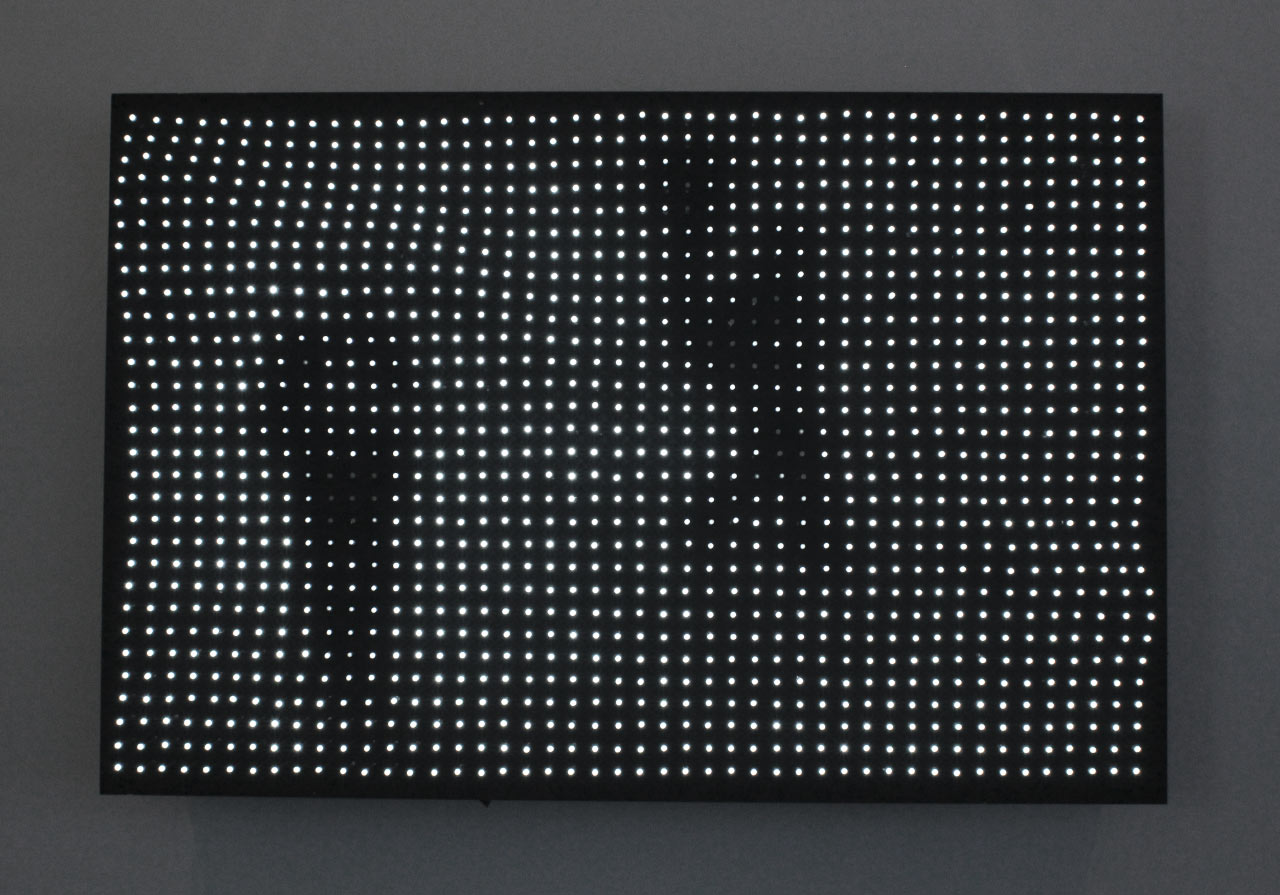
\includegraphics[width=0.8\textwidth]{./04-figuras/jim_campbell}
    \label{fig:jim_campbell}
\end{figure}
\vspace*{-0,9cm}
{\raggedright \fonte{Disponível em: <https://design-milk.com/pixelated-led-art-jim-campbell/>. Acesso em: 22 mar. 2018}}\\

Do ponto de vista da propagação da luz, o cubo branco tende a não ser o cenário ideal para exibição deste tipo de obra. Além disso, \citeonline[p. 40]{soares}, afirma que "a maioria dos autores que trabalham com arte e tecnologia procuram o espaço do cubo preto como espaço expositivo. Neste espaço o que interessa é um novo ver, um espanto com a imagem". Diz ainda que o nome cubo preto para este tipo de exposição surge em contraposição ao cubo branco, criado por Brian O'Doherty, num ensaio publicado pela revista Artforum em 1976, fazendo alusão ao espaço das galerias de arte, com paredes brancas, sem janelas isolando o espetador num meio aparentemente atemporal. A ideia do cubo preto surge como ambiente ideal para propagação da luz e é também uma forma de imersão no interior da mente do artista.


\section{  }

Para compreender a cor é necessário percebê-la como um todo, como um conjunto de fatores de onde ela deriva. Para se investigar sua origem é necessário compreender que a cor nada é, sem a luz, pois, sem a luz, perdemos de vista qualquer sinal visual de uma determinada cor. E se, para ter a cor, é necessária a luz como fator reagente, considera- se que a cor, em sua propriedade, é formada pela luz. \cite[p. 55]{henno}


A cor se deriva da luz, seja ela natural ou artificial. Com pouca luz, pouca ou nenhuma cor é presente. Com muita luz aparecem muitas cores. Uma luz forte produz uma cor intensa (MORIOKA; STONE, 2006, p. 10). \cite[p.56]{henno}

Desta forma, de acordo com o que foi investigado, a luz é radiação. E a cor uma transformação da luz, determinada por uma mistura de radiações simples. Essas radiações são classificadas segundo o seu comprimento de onda, que decresce imperceptivelmente do vermelho ao violeta. Com isso é possível comprovar que o elemento determinante para a manifestação da cor é a luz, pois sem ela não há radiação e consequentemente não identificaríamos a cor. \cite[p.56]{henno}

A cor, como fonte luminosa, levando em conta Plaza (1986, p.133), manifesta-se sem significado, por ser ela pura “forma-luz”. Ela é um signo em estado de abertura para interpretações, passíveis de uma multiplicidade de significados. No entanto, complementa o autor, a cor pode passar a ser suporte de significação quando aliada a formas analógicas, o que resulta numa organização de linguagem mais complexa. \cite[p.60]{henno}


A luz desde os primórdios da humanidade, quando o homem descobria o fogo sempre desencadeou fascínio. Esse deslumbramento permanece até os dias de hoje. O homem continuamente trabalha no sentido de dominar a luz e dela se apropriar. Aliado ao desenvolvimento da ciência e da tecnologia, o homem de hoje tem condições de gerar e projetar a luz artificialmente em lugar de restringir-se aos meios naturais. Ao apropriar da luz, o homem controla as emissões cromáticas a ela vinculadas, a partir de filtros ou de dispositivos tecnológicos específicos. \cite[p.73]{henno}

O artista das novas mídias dispõe, hoje, de ferramentas que lhe possibilitam projetar através da luz. E dessa forma, no caso da luz como fonte de emissão ou projeção, o artista controla os dispositivos de luz, trabalhando poeticamente no momento em que confere um sentido à sua obra. Com o passar dos anos, os limites desses dispositivos se dissipam o que permite a interação homem e luz cada vez mais próxima. O reflexo dessa relação cada vez maior com os dispositivos técnicos, propiciou uma abertura crescente da obra: o artista pode trabalhar em conjunto com o espectador / ator na construção de seu sentido. \cite[p.73]{henno}

Com as novas tecnologias eletrônicas instauram-se diferentes possibilidades de participação do público na arte. O artista passa a ter em mãos uma grande diversidade de dispositivos para trabalhar com a luz. Esses métodos tecnológicos continuamente possibilitam o uso na arte que explora o campo sensorial. A participação de quem contempla a arte é potencializada de maneira inovadora e sem limites.  \cite[p.86]{henno}

O computador passa a ser um meio que gerencia as trocas de informação e sentidos. \cite[p.112]{henno}

Atualmente, a cor como fonte luminosa artificial quase não enfrenta barreiras em sua manipulação física: pode ser trabalhada a partir de equipamentos e interfaces mais sofisticadas e sensoriais, o que permite um acesso e uma interação mais efetiva do receptor. \cite[p.112]{henno}

De acordo com Poissant (2009, p.76-77), uma das alternativas para envolver o espectador cada vez mais no processo de criação seria a de levar a obra para fora dos espaços fechados como a galeria, por exemplo. No meio externo não existe o silêncio, não existem atitudes pre-concebidas, não existe a intenção. A obra sai do museu e da galeria para ficar próxima do público geral. Desta forma, levando-se em conta que o recorte desta pesquisa se dá no uso da cor por fonte luminosa, entendemos que para viabilizar a percepção da obra, esta deve ser atualizada durante o período da noite, quando há pouca ou nenhuma luminosidade. Desta forma, a intensidade das cores é maior e mais perceptível devido ao contraste com a escuridão. A luz colorida quando utilizada em locais externos de pouca ou quase nula iluminação natural impressiona e chama a atenção de um observador passante. O contraste da cor como informação luminosa em face da escuridão da noite estabelece comunicação com o observador seduzindo-o pelos sentidos que tal cor suscita. \cite[p.125]{henno}







